\chapter{Análisis y diseño del sistema}

En este capítulo se expone el análisis de requisitos funcionales del sistema acordado con la empresa. A continuación se presenta la arquitectura software final que tiene el sistema y se explica lo relevante respecto a la base de datos que se utiliza para la aplicación. Por último se muestra la interfaz del usuario final.

\section{Requisitos del sistema}

% Tabla con los requisitos del sistema

\ref{tab:etiqueta_tabla}

\begin{table}[!h]
\centering
\begin{tabular}{|p{1cm}|p{14cm}|}
	\hline
	\textbf{ID} & \textbf{Requisito} \\
	\hline
	RF-1 	& 	Un usuario deberá iniciar sesión en el sistema utilizando usuario, contraseña y puesto	\\
	\hline
	RF-2	&	Un usuario podrá cerrar su sesión	\\
	\hline
	RF-3	&	El sistema mostrará al usuario un carrusel con el listado de alertas y su información necesaria de la planta seleccionada \\
	\hline
	RF-4	&	El sistema mostrará al usuario el plano de la planta seleccionada \\
	\hline
	RF-5	&	El sistema mostrará al usuario el listado de plantas y permitirá seleccionar una de ellas	\\
	\hline
	RF-6	&	El sistema mostrará al usuario el listado de alertas pendientes sin filtrado por planta con la información básica \\
	\hline
	RF-7	&	El sistema mostrará al usuario el número total de alarmas y presencias \\
	\hline
	RF-8	&	El sistema permitirá al usuario navegar en la aplicación mediante un menú lateral \\
	\hline
	\end{tabular}
\caption{Requisitos funcionales del sistema}
\label{tab:etiqueta_tabla}
\end{table}

\section{Arquitectura software del sistema}

% Explicar la arquitectura final del sistema

% Hacer referencia al Anexo donde se expliquen las alternativas que se plantearon

Para ver las relaciones entre el software y su entorno (dónde se despliega y ejecuta) se utiliza una vista de distribución estilo despliegue. Se puede ver en la \textit{Figura 2.1}. \newline

\begin{figure}[!h]
    \centering
    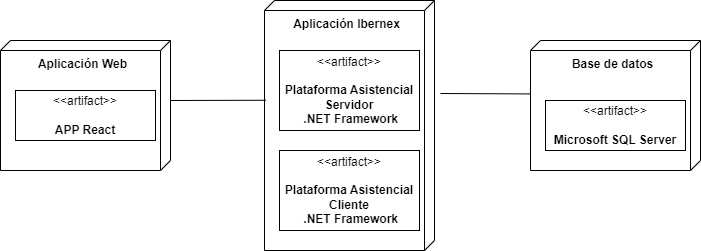
\includegraphics[width=0.8\textwidth,height=6cm]{Imagenes/Arquitectura_Sistema}
    \caption{Diagrama de despliegue}
    \label{fig:despliegue}
\end{figure}

La arquitectura completa respecto a lo que ha estado relacionado con el proyecto es la que se ve en la figura. No obstante lo que se ha implementado ha sido completamente la aplicación web y por otro lado se ha modificado y añadido funcionalidad a la Plataforma Asistencial Servidor de la aplicación de Ibernex. \newline

El ámbito del despliegue del sistema será en una red de área local (LAN) ya que serviría para una residencia u hospital en el que se instalaría el sistema configurando la base de datos correspondiente a la información de los pacientes del centro. \newline


TODO: Terminar de explicar la arquitectura final del sistema consultando con Carlos para hacerlo correctamente respecto a la parte de Ibernex\\

TODO: Hacer referencia al Anexo donde se expliquen las alternativas que se plantearon


\section{Base de datos}

% Explicar qué partes de la base de datos utilizo de su sistema y con diagramas

TODO: explicar qué tablas de la base de datos utilizo de su sistema y adjuntaré  diagramas credos con la aplicación Microsoft SQL Server Management. \\

\section{Interfaz de usuario}

% Poner la interfaz final del usuario cuando esté terminada

TODO: Poner la interfaz final del usuario cuando esté terminada
